\item \textbf{Walk/non-Walk Classification: Train an HMM model to detect the activity ‘Walk’ using users 1-10 for training. Then, use the model to detect ‘walk’ activity patterns in the data from users 11-15. The goal here is to label during which parts of the data the user were walking. You can adjust the selection criteria by varying the likelihood threshold. Compute the system performance/accuracy across different thresholds (hint: explore ROC curves).}

This question is a learning problem. Figure \ref{} indicates the pipeline of my solution. For pre-processing part, we used \emph{re-sampling function} to resize all observations. This could remove the effect of zero padding. After that, 9 varies features were extracted from each each observation signal. We also considered a window with size of 256 samples and overlap portion of 20 percent. Based the observation signals, the mean and variance of signal were calculated as features. Also we found 6 peak values in the Short-time Fourier transform, with the same algorithm used in tutorial. figure \ref{} show the peak values for a subset of a signal.
\begin{figure}[H]
    \centering
    \begin{minipage}[b]{1\textwidth}
        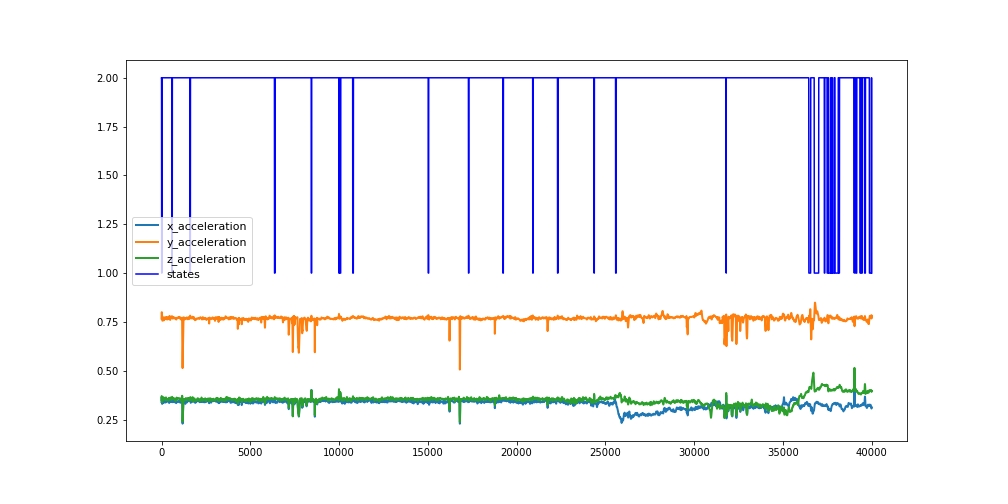
\includegraphics[width=\textwidth]{manuscript/src/figures/Ass3/Ass3_Q2_states_user_10N.png}
    \end{minipage}
    \caption{The normalized signals of x, y, and z for participant 11 and ‘Standing  Up,  Walking  and  Going  up-down  stairs’ activity. The dark blue signal indicates the different states.}
    \label{fig:Ass3_Q2_states_user_10N}
\end{figure}

The output of this section is a matrix with dimension of $3 \times 411 \times 9$ for each activity. 
Then features of each observation (x, y, and z) concatenated to each other to produce a matrix of $411 \times 27$ for each user activity. finally, features were separated based on their activities. the shape of the final array is $15 \times 411 \times 27$; where 15, 411, and 27 indicate number of users, windows, and features respectively.  

In classification part, the array was divided into train and test array. Based on the question, we used users 1 to 10 for training and others for test. Also we set the state variable as loop variable to find the effect of the HMM state in accuracy.

Because we have only one HMM model that was trained for walking activity, the output is the probability. this probability shows whether or not the test features belonged to the this activity. To find the best threshold, we used a \emph{for loop}. The results of this model are illustrated below.  


\begin{table}[H]
\centering
\caption{The results of HMM for different states and thresholds.}
\label{tab:Q2_results}
\begin{tabular}{l}
\toprule
    Test accuracy of 2 states HMM for threshold -10000 : $64.29\%$ \\
    Test accuracy of 2 states HMM for threshold -20000 : 57.14\% \\
    Test accuracy of 2 states HMM for threshold -30000 : 57.14\% \\
    Test accuracy of 2 states HMM for threshold -40000 : 50.00\% \\
    Test accuracy of 2 states HMM for threshold -50000 : 50.00\% \\
    Test accuracy of 2 states HMM for threshold -60000 : 71.43\% \\
    Test accuracy of 2 states HMM for threshold -70000 : \textbf{85.71\%}\\
    Test accuracy of 3 states HMM for threshold -10000 : 64.29\% \\
    Test accuracy of 3 states HMM for threshold -20000 : 50.00\% \\
    Test accuracy of 3 states HMM for threshold -30000 : 50.00\% \\
    Test accuracy of 3 states HMM for threshold -40000 : 42.86\% \\
    Test accuracy of 3 states HMM for threshold -50000 : 50.00\% \\
    Test accuracy of 3 states HMM for threshold -60000 : 50.00\% \\
    Test accuracy of 3 states HMM for threshold -70000 : 57.14\% \\
    Test accuracy of 4 states HMM for threshold -10000 : 57.14\% \\
    Test accuracy of 4 states HMM for threshold -20000 : 57.14\% \\
    Test accuracy of 4 states HMM for threshold -30000 : 50.00\% \\
    Test accuracy of 4 states HMM for threshold -40000 : 57.14\% \\
    Test accuracy of 4 states HMM for threshold -50000 : 50.00\% \\
    Test accuracy of 4 states HMM for threshold -60000 : 50.00\% \\
    Test accuracy of 4 states HMM for threshold -70000 : 57.14\% \\
    Test accuracy of 5 states HMM for threshold -10000 : 64.29\% \\
    Test accuracy of 5 states HMM for threshold -20000 : 64.29\% \\
    Test accuracy of 5 states HMM for threshold -30000 : 64.29\% \\
    Test accuracy of 5 states HMM for threshold -40000 : 64.29\% \\
    Test accuracy of 5 states HMM for threshold -50000 : 57.14\% \\
    Test accuracy of 5 states HMM for threshold -60000 : 57.14\% \\
    Test accuracy of 5 states HMM for threshold -70000 : 57.14\% \\
\bottomrule

\end{tabular}
\end{table}




 
